\documentclass[a4paper, 11pt]{article}
\usepackage{comment} % enables the use of multi-line comments (\ifx \fi)
\usepackage{lipsum} %This package just generates Lorem Ipsum filler text.
\usepackage{fullpage} % changes the margin
\usepackage[brazilian]{babel}
\usepackage[utf8]{inputenc}
\usepackage[T1]{fontenc}
\usepackage{graphicx}

\begin{document}
%Header-Make sure you update this information!!!!
\noindent
\large\textbf{Melhoria de Processo de Software / Segundo trabalho}\\
Lucas Albuquerque Medeiros de Moura \hfill 11/0015568 \\
Luciano Prestes Cavalcanti \hfill 11/0035208

\section*{Resumo do trabalho}

Este trabalho visa explicitar o processo de desenvolvimento para a evolução do
software Noosfero no contexto do Laboratório Avançado de Produção Pesquisa e
Inovação em Software (LAPPIS).

\section*{Introdução}

O Noosfero pode ser descrito como plataforma web com o foco de permitir a
customização de redes sociais, visando desde a criação de blogs a até mesmo
agenda de eventos. Tal software é atualmente usado pela Universidade de São
Paulo para gerencimento de algumas de suas disciplinas e até mesmo pelo
SERPRO.

No contexto do LAPPIS, o Noosfero é usado para prover uma rede social para o
novo portal de software público. O intuito desse portal é provar uma
plataforma única de gerenciamento de softwares livre do governo, visando desde
prover um repositório de código fonte a até mesmo prover um meio para
interação da comunidade de um dado software livre. O Noosfero, dessa forma, é
responsável pela configuração desse ambiente de interação entre os membros de
uma comunidade.

Com isso em mente, o laboratório LAPPIS tem como motivação a criação de um
processo que vise tanto a manutenção de um fork do Noosfero para o contexto do
novo portal do software público e também estar alinhado e presente com o
desenvolvimento da versão principal do Noosfero. Considerando que o LAPPIS
baseia seu processo em técnicas propostas pela metodologia ágil, onde todo o
processo de desenvolvimento é encapsulado em uma sprint de trabalho, que
normalmente tem duração de duas semanas.

Sendo assim, durante uma sprint, o processo de desenvolvimento usado segue as
seguintes atividades:

\begin{figure}[ht!]
\centering
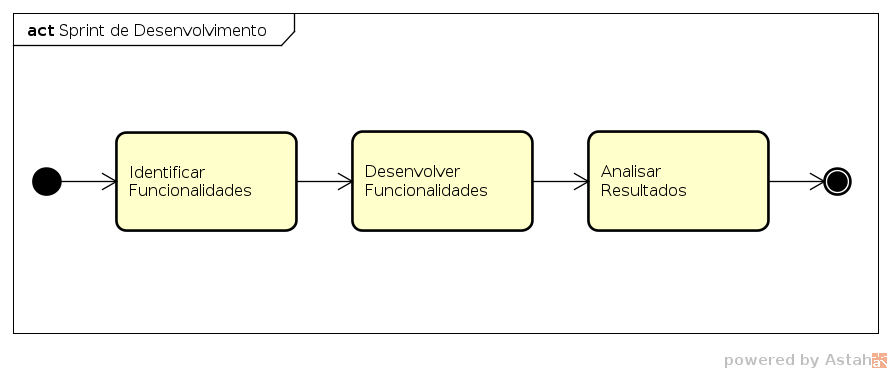
\includegraphics[width=150mm]{sprint_devel.png}
\caption{Processo de Desenvolvimento de uma Sprint \label{overflow}}
\end{figure}

O objetivo desse processo é então, basicamente, a criação de novas
funcionalides para o Noosfero no contexto do software público de forma
dinâmica e de rápida assimilação pelo time.

Com o processo minimamente explicado, pode-se então explicar como esse
documento será estruturado. Esse documento é composto por duas sessões,
Desenvolvimento e Considerações finais. A sessão de Desenvolvimento é usado
para o detalhamento do objetivo e das atividades de cada etapa do processo,
além de explicar como tais atividades são detalhadas e quais ferramentas são
usadas para o acompanhamento do processo.


\section*{Desenvolvimento}

Considerando as etapas levantadas na seção anterior, é necessário descrever
melhor o motivo e as atividades relacionadas a cada uma delas. Esta seção visa
então realizar tal papel, além de mostrar em linhas gerais quais as
ferramentas e papéis usados para o gerenciamento do processo como um todo.

\subsection*{Identificar Funcionalidades}

Esta etapa do processo é usada para selecionar quais tarefas precisam ser
realizadas dentro da sprint, levando em consideração a prioridade de cada uma
das tarefas e a composição do time. As atividades dessa etapa são apresentadas
na figura a seguir:

\begin{figure}[ht!]
\centering
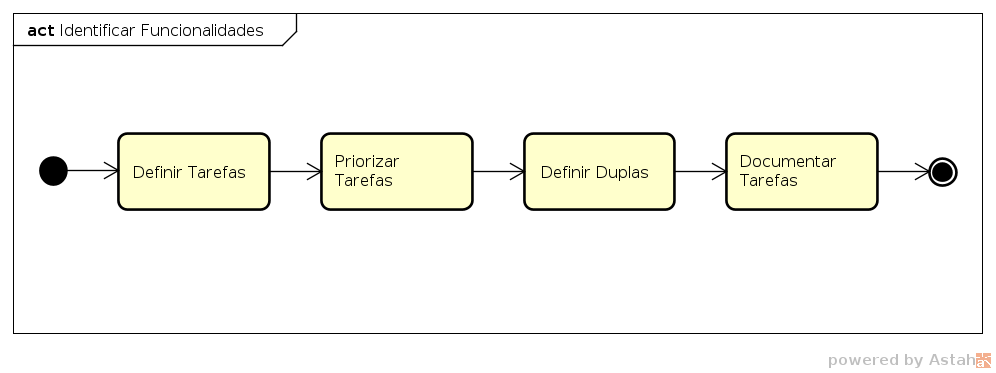
\includegraphics[width=150mm]{ident_func.png}
\caption{Identificar Funcionalidades\label{overflow}}
\end{figure}

\pagebreak

A tabela à seguir descreve as atividades necessárias para a execução dessa etapa:

\begin{table}[h]
    \resizebox{\textwidth}{!}{\begin{tabular}{|l|l|}
		\hline
        Atividade          & Função \\ \hline
        Definir tarefas    & \parbox{10cm}{Definir quais são as atividades que
precisam ser realizadas para a sprint, ou até mesmo, em algum momento do
projeto.\\} \\ \hline
        Priorizar tarefas  & \parbox{10cm}{Com as tarefas definidas, deve-se
priorizar quais são as principais tarefas que devem ser desempanhadas na
duração da sprint. Essa tarefa deve ser realizada em conjunto com todo o time
relacionado ao Noosfero.\\}\\ \hline
        Definir duplas     & \parbox{10cm}{Com as tarefas priorizadas, deve-se
definir quais duplas devem ser responsáveis pelo desenvolvimento de cada
tarefa.\\} \\ \hline
        Documentar tarefas & \parbox{10cm}{Com as duplas definidas, cada dupla
deve documentar suas tarefas e documentar qualquer subtarefa relacionada a
mesma. Além disso, a dupla também deve ser responsável por definir o
critério de aceitação de uma dada tarefa.\\} \\ \hline
	  \end{tabular}}
    \caption{Atividades relacionadas a etapa de Identificar funcionalidades}
    \label{tab:atividades_identificar}
\end{table}

\subsection*{Desenvolver funcionalidade}

Esta etapa do processo visa realizar uma tarefa proposta. Apesar da abordagem
de como abordar uma tarefa seja responsabilidade da dupla destinada a
realizar tal tarefa, existem uma categorização informal de como tratar alguns
tipos de tarefas:

\begin{itemize}
    \item \textbf{Funcionalidades para o SPB:} Quando uma funcionalidade deve
        ser desenvolvida só para o contexto do SPB, a dupla responsável deve
        fazer as alterações somente no fork do Noosfero para o SPB. Para este
        tipo de tarefa, não é explicitamente necessário a interação da dupla
        com os mantenedores do Noosfero, mas obviamente, tal interação não é
        restrita.
    \item \textbf{Funcionalidades para o Noosfero:} Quando uma funcionalidade
        proposta pode empactar usuários do Noosfero que não estão só
        relacionados ao contexto do SPB, tal funcionalidade ou modificação
        deve ser feita no repositório principal do Noosfero. Para isso, é
        necessário que a dupla se organize para interagir diretamente com os
        mantenedores do Noosfero, pois tal interação ocorre normalmente de
        forma não presencial.
    \item \textbf{Correção de bugs:} Neste tipo de tarefa, normalmente
        tenta-se alocar os responsáveis iniciais pela tarefa que gerou um
        bug. Caso isso não seja possível, deve-se minimanete tentar entrar em
        contato com a dupla original e tentar nortear o que pode estar
        causando o bug, com o intuito de poupar esforço inicial de encontrar
        onde está o bug, e sim focar em consertar o problema.
\end{itemize}

Apesar desses três tipos de tarefas principais, existem também tarefas
relacionadas a documentação e tradução do Noosfero. Entretanto, tais tarefas
seguem o mesmo fluxo de atividades que será detalhada a seguir, e não carecem
de nenhuma explicação mais detalhada.

Considerando os tipos de tarefas realizadas pela equipe, tornou-se necessário
a descrição das seguintes atividades para esta etapa do processo:

\begin{figure}[ht!]
\centering
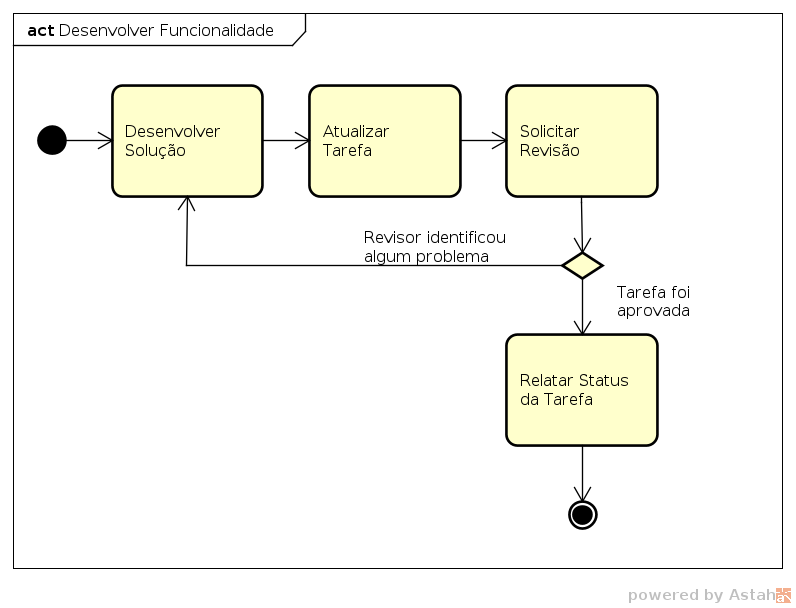
\includegraphics[width=150mm]{devel_func.png}
\caption{Desenvolver Funcionalidade\label{overflow}}
\end{figure}

\pagebreak

Onde a tabela a seguir apresenta os detalhes de cada tarefa citada na figura
a cima.

\begin{table}[h]
    \resizebox{\textwidth}{!}{\begin{tabular}{|l|l|}
		\hline
        Atividade          & Função \\ \hline
        Desenvolver solução    & \parbox{10cm}{Esta atividade está relacionada
        ao trabalho efetivo para implementar uma solução para uma dada tarefa
        da dupla.\\} \\ \hline

        Atualizar tarefa  & \parbox{10cm}{Conforme o andamento da tarefa, a
        dupla deve sempre atualizar como está o andamento das atividades, como
        por exemplo, o que já está terminado e o que está sendo feito.\\}\\
        \hline

        Solicitar revisão     & \parbox{10cm}{Com a tarefa totalmente
        concluída, a dupla deve pedir para que outros membros do time ou,
        dependendo do tipo de tarefa sendo desenvolvida, um mantenedor do
        Noosfero, que revise a solução desenvolvida. A dupla pode apontar
        quem ela acha melhor para revisar tal tarefa, mas tal apontamento
        não é fixo e pode ser alterado de acordo com as necessidades do time.
        Caso o revisor da tarefa encontre algum problema na solução
        encontrada, a dupla deve voltar a ativide de desenvolver solução e
        corrigir os problemas apontados.\\}\\ \hline

        Relatar status da tarefa & \parbox{10cm}{Durante a execução da sprint,
        a dupla deve relatar o andamento de sua tarefa. Tal relato não é feito
        só para o time do Noosfero propriamente dito, mas sim para para todo o
        time do SPB, visando que todos os membros estejam alinhados quanto ao
        objetivo da sprint e dos projetos ao seu redor.\\} \\
		\hline
	\end{tabular}}
    \caption{Atividades relacionadas a etapa de Desenvolver funcionalidades}
    \label{tab:atividades_desenvolver}
\end{table}

\pagebreak

\subsection*{Analisar resultados}

Esta etapa do projeto acontece quando a sprint chega ao seu término. Dessa
forma, esta etapa visa entender o que foi realizado na sprint, se alguma
tarefa na sprint não foi concluída, e para entender o que pode ser melhorado
na próxima sprint.

Dessa forma, esta etapa possui as seguintes atividades:

\begin{figure}[ht!]
\centering
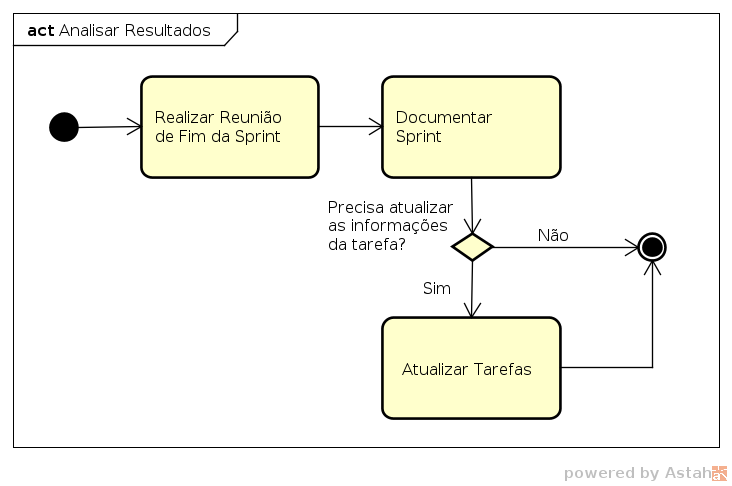
\includegraphics[width=150mm]{check_result.png}
\caption{Analisar Resultados\label{overflow}}
\end{figure}

\pagebreak

Os detalhes das atividades do processo de analise de resultados é descrito na
tabela a baixo:

\begin{table}[h]
    \resizebox{\textwidth}{!}{\begin{tabular}{|l|l|}
		\hline
        Atividade          & Função \\ \hline
        Realizar reunião de fim da sprint& \parbox{10cm}{Esta atividade
        acontece ao término de uma sprint, onde ambas as tarefas encerradas e
        pendentes são reportadas para todo o time. Além disso, nessa reunião
        também é levantado os problemas encontrados durante a execução da
        sprint e o  que o time pode fazer para mitigar tais dificuldades no
        próximo ciclo de desenvolvimento.\\} \\ \hline

        Documentar sprint& \parbox{10cm}{Após a reunião de término, o time
        deve documentar o que foi realizado na sprint. Onde toda a
        documentação é feita na wiki do projeto, relatando o que foi foi
        realizado e o que ainda precisa ser feito ser feito.\\}\\ \hline

        Atualizar tarefas& \parbox{10cm}{Dependendo da tarefa, a sua
        documentação pode carecer de atualização ao término de uma sprint. Por
        exemplo, caso o seu motivo de existir tenha sido alterado ou até mesmo
        se seus critérios de aceitação forem alterados. Dessa forma, a dupla
        responsável pela tarefa deve atualizar tais informações.\\}\\ \hline
	\end{tabular}}
    \caption{Atividades relacionadas a etapa de Analisar Resultados}
    \label{tab:atividades_desenvolver}
\end{table}

\subsection*{Ferramentas}

Para gerenciar o processo criado para o projeto SPB, as seguintes ferramentas
são utilizadas:


\begin{table}[h]
    \resizebox{\textwidth}{!}{\begin{tabular}{|l|l|}
		\hline
        Ferramenta          & Função \\ \hline
        Gitlab & \parbox{10cm}{Ferramenta usada como repositório de código
        fonte para o Noosfero, além de gerenciar as tarefas que são
        desenvolvidas e também a wiki do projeto, suportando o acompanhamento
        das sprints. \\} \\ \hline

        IRC & \parbox{10cm}{Usado para comunicação entre membros do time e com
        os mantenedores do Noosfero.\\}\\ \hline

        Lista de email& \parbox{10cm}{Usado para comunicação mais detalhada
        sobre andamento da sprint ou problemas no decorrer da mesma.\\}\\ \hline
	\end{tabular}}
    \caption{Atividades relacionadas a etapa de Desenvolver funcionalidades}
    \label{tab:atividades_desenvolver}
\end{table}

\subsection*{Papéis}

No contexto do projeto SPB, existem quatro papéis distintos no processo:

\begin{itemize}
    \item \textbf{Desenvolvedor:} Responsável pelo desenvolvimento de
        funcionalidade e correção de problemas.
    \item \textbf{Couch:} Responsável por ajudar o time a se organizar e ser
    um ponto central quanto a questionamentos sobre andamentos de tarefa.
    \item \textbf{Meta couch:} Responsável por fazer a ponte entre os
    diferentes time do projeto. Muitas vezes, é alocado em tarefas de
    integração entre as ferramentas.
    \item \textbf{Sênior:} Desenvolvedor mais experiente no projeto.
    Normalmente recebe as funcionalidades mais complexas e ajuda o time
    quanto a dúvidas técnicas.
\end{itemize}

Vale ressaltar, que mesmo com essa diferença de papéis, todos os membros do
projeto são responsáveis pelo desenvolvimento, os papéis apenas tem abordagens
diferentes quanto a isso.


\subsection*{Integração com outros processos}

Considerando que o portal do software público é composto por várias
ferramentas integradas, o processo usado pelo Noosfero interage frequentemente
com outros processos de outros softwares do projeto. Quando isso é necessário,
o time como um todo levanta quais tarefas devem ser feitas em conjunto, ou
seja, que precisam do Noosfero e de outro software. Dessa forma, membros de
ambos os times são escolhidos para formar uma dupla e resolver o problema.

Ess tipo de integração ocorre frequentemente quando é necessário empacotar o
Noosfero para deploy ou então adicionar uma funcionalidade no Noosfero que
impacta outro software relacionado.

Dessa forma, o processo de integração funciona de forma similar ao já
levantado, com a única diferença que a primeira etapa do processo não é
realizada apenas por membros do time do Noosfero e sim por esses membros e de
outros times.

\section*{Considerações finais}

O processo adotado no projeto SPB já propiciou alguns resultados louváveis
para o Noosfero e para o SPB como um todo. Atualmente, o Noosfero já possui
uma API desenvolvida basicamente pelo time do projeto usando tal processo.
Além disso, novas funcionalidades foram adicionadas ao Noosfero, como a
possibilidade de permitir aos usuários realizarem uma avaliação das
comunidades cadastradas na plataforma.

Por fim, o processo de integração também está funcionando razoavelmente bem,
pois hoje o Noosfero possui integração de login e perfil de usuário em outros
softwares do projeto, uma funcionalidade que surgiu através de uma necessidade
do software público e que adicionou ao Noosfero um plugin que permite essa
integração de login através de outro software, e esse plugin pode ser
utilizado em qualquer outro projeto que use o Noosfero.

Entretanto, apesar desses pontos positivos, o processo ainda tem problemas
relacionados ao ambiente de desenvolvimento. Apesar de hoje configurar e
preparar ambiente requerer menor esforço manual, existem ainda algumas etapas
que precisam ser automatizadas e são constatemente levantadas pelo time.

Para isso, for criado um time responsável por essa tarefa de melhorar a
configuração de ambientes do SPB. Apesar de que algumas melhorias já se
tornaram visíveis, principalmente quanto ao uso de ambiente de homologação, o
processo usado atualmente ainda precisa refletir melhor as questões de
automação sendo desenvolvidas, para permitir que todos os membros do projeto
se beneficiem dela.

\begin{thebibliography}{9}
\bibitem{Robotics} Fred G. Martin \emph{Robotics Explorations: A Hands-On
Introduction to Engineering}. New Jersey: Prentice Hall.
\bibitem{Flueck}  Flueck, Alexander J. 2005. \emph{ECE 100}[online]. Chicago:
Illinois Institute of Technology, Electrical and Computer Engineering
Department, 2005 [cited 30
August 2005]. Available from World Wide Web:
(http://www.ece.iit.edu/~flueck/ece100).
\end{thebibliography}

\end{document}
